\begin{name}
{Sở GD Nam Định}
{ĐỀ THI THỬ TỐT NGHIỆP THPT--NĂM 2022 }
\end{name}
\Opensolutionfile{ans}[sonamdinh-]

\begin{ex} 
 Môđun của số phức $z=4+2 i$ bằng
\choice 
 { 20 } 
 { 6 } 
 { $2 \sqrt{5}$} 
 { 8 }
\end{ex} 
 
\begin{ex} 
 Trong không gian $O x y z$, mặt cầu $(S):(x-2)^{2}+(y-2)^{2}+(z+1)^{2}=16$ có bán kính bằng
\choice 
 { 4 } 
 { 16 } 
 { 2 } 
 { 9 }
\end{ex} 
 
\begin{ex} 
 Điểm nào dưới đây thuộc đồ thị của hàm số $y=2 x^{4}-x^{2}-1$ ?
\choice 
 { $E(-1 ; 0)$} 
 { $F(-1 ; 2)$} 
 { $K(-1 ; 4)$} 
 { $D(-1 ; 1)$}
\end{ex} 
 
\begin{ex} 
 Diện tích $S$ của mặt cầu bán kính $r$ được tính theo công thức nào dưới đây?
\choice 
 { $S=\pi r^{2}$} 
 { $S=\frac{4}{3} \pi r^{2}$} 
 { $S=2 \pi r^{2}$} 
 { $S=4 \pi r^{2}$}
\end{ex} 
 
\begin{ex} 
 Trên khoảng $(-\infty ;+\infty)$, họ nguyên hàm của hàm số $f(x)=5^{x}$ là
\choice 
 { $5^{x} \ln 5+C$} 
 { $\frac{5^{x}}{\ln 5}+C$} 
 { $5^{x}+C$} 
 { $\frac{5^{x+1}}{x+1}+C$}
\end{ex} 
 
\begin{ex} 
 Cho hàm số $f(x)$ có bảng xét dấu của đạo hàm như sau:
\\ \centerline{

\begin{tikzpicture}
\tkzTabInit[nocadre,lgt=1.2,espcl=2.2]
{$x$ /.6,$f'(x)$ /.6}
{$-\infty$,$1$,$2$,$3$,$4$,$+\infty$}
\tkzTabLine{,-,$0$,+,$0$,+,$0$,-,$0$,+,}
%\tkzTabVar{-/ $-\infty$ ,+/$3$,-/$-1$,+/$3$,-/$-\infty$}
\end{tikzpicture}
}\\
Số điểm cực trị của hàm số đã cho là
\choice 
 { 4 } 
 { 3 } 
 { 2 } 
 { 5 }
\end{ex} 
 
\begin{ex} 
 Tập nghiệm của bất phương trình $\left(\frac{1}{2}\right)^{x}>1$ là
\choice 
 { $(0 ;+\infty)$} 
 { $\mathbb{R}$} 
 { $(-\infty ; 0)$} 
 { $(2 ;+\infty)$}
\end{ex} 
 
\begin{ex} 
 Cho khối chóp có diện tích đáy $B=6$ và chiều cao $h=7$. Thể tích của khối chóp đã cho bằng
\choice 
 { 42 } 
 { 126 } 
 { 14} 
 { 56 }
\end{ex} 
 
\begin{ex} 
 Tập xác định của hàm số $y=x^{\sqrt{3}}$ là
\choice 
 { $\mathbb{R}$} 
 { $(0 ;+\infty)$} 
 { $\mathbb{R} \backslash\{0\}$} 
 { $[0 ;+\infty)$}
\end{ex} 
 
\begin{ex} 
 Nghiệm của phương trình $\log _{3}(x+5)=2$ là
\choice 
 { $x=4$} 
 { $x=3$} 
 { $x=1$} 
 { $x=-3$}
\end{ex} 
 
\begin{ex} 
 Nếu $\int_{0}^{1} f(x) d x=2$ và $\int_{0}^{1} g(x) d x=-3$ thì $\int_{0}^{1}[2 f(x)+g(x)] d x$ bằng
\choice 
 { 7 } 
 { $-1$} 
 { $-4$} 
 { 1 }
\end{ex} 
 
\begin{ex} 
 Cho số phức $z_{1}=2+3 i$ và số phức $z_{2}=3-2 i$. Phần thực của số phức $z_{1}+z_{2}$ bằng
\choice 
 { 1 } 
 { 0 } 
 { 5 } 
 { $\sqrt{13}$}
\end{ex} 
 
\begin{ex} 
 Trong không gian $O x y z$, cho mặt phẳng $(\alpha): x-2 y+3 z-4=0$. Vectơ nào dưới đây là một vectơ pháp tuyến của mặt phẳng $(\alpha)$ ?
\choice 
 { $\overrightarrow{n_{2}}=(1 ;-2 ; 3)$} 
 { $\vec{n}_{1}=(1 ; 2 ; 3)$} 
 { $\overrightarrow{n_{4}}=(-2 ; 3 ;-4)$} 
 { $\overrightarrow{n_{3}}=(1 ; 3 ; 4)$}
\end{ex} 
 
\begin{ex} 
 Trong không gian $O x y z$, cho hai vectơ $\vec{a}=(1 ; 3 ; 2)$ và $\vec{b}=(3 ; 1 ; 2)$. Tọa độ của vectơ $\vec{a}+2 \vec{b}$ là
\choice 
 { $(7 ; 4 ; 4)$} 
 { $(7 ; 5 ; 6)$} 
 { $(5 ; 5 ; 4)$} 
 { $(4 ; 4 ; 4)$}
\end{ex} 
 
\begin{ex} 
 Trong mặt phẳng tọa độ $O x y$, cho $M(2 ;-3)$ là điểm biểu diễn số phức $z$. Phần ảo của số phức $z$ là
\choice 
 { $\sqrt{13}$} 
 { 2 } 
 { $-3 i$} 
 { $-3$}
\end{ex} 
 
\begin{ex} 
 Tiệm cận ngang của đồ thị hàm số $y=\frac{3 x-2}{x+2}$ là đường thẳng có phương trình:
\choice 
 { $y=3$} 
 { $y=-2$} 
 { $y=-1$} 
 { $y=-3$}
\end{ex} 
 
\begin{ex} 
 Với mọi số thực dương $x, \log _{3}\left(\frac{x^{3}}{3}\right)$ bằng
\choice 
 { $3 \log _{3} x-1$} 
 { $\log _{3} x-1$} 
 { $\log _{3} x$} 
 { $3 \log _{3} x+1$}
\end{ex} 
 
\begin{ex} 
 \immini[thm]{Hàm số nào dưới đây có đồ thị như đường cong trong hình vẽ bên?
\choice 
 { $y=x^{2}-2 x-2$} 
 { $y=x^{3}-3 x-2$} 
 { $y=x^{4}-4 x^{2}+2$} 
 { $y=-x^{4}+4 x^{2}+2$}}
 {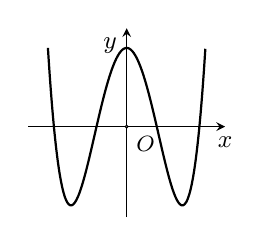
\begin{tikzpicture}[scale=.5]
\draw[-stealth] (-2.5,0) -- (2.5,0) node[below]{\small $x$};
\draw[-stealth] (0,-2.3) -- (0,2.5) node[below left]{\small $y$};
\draw[thick,smooth,samples=100] plot[domain=-2:2](\x,{(\x)^4-4*(\x)^2+2});
\draw [fill=white,draw=black] (0,0) circle (1pt)node[below right]{\footnotesize $O$};
\end{tikzpicture}
 }
\end{ex} 
 
\begin{ex} 
 Trong không gian $O x y z$, cho đường thẳng $d:\left\{\begin{array}{l}x=1-2 t y=3+t z=-1-t\end{array}\right.$. Đường thẳng $d$ đi qua điểm nào dưới đây?
\choice 
 { $E(5 ; 1 ; 1)$} 
 { $H(1 ; 3 ; 1)$} 
 { $T(-2 ; 1 ;-1)$} 
 { $Q(-5 ; 0 ; 1)$}
\end{ex} 
 
\begin{ex} 
 Với $n$ là số nguyên dương và $k$ là số tự nhiên, $k \leq n$, công thức nào dưới đây đúng?
\choice 
 { $A_{n}^{k}=\frac{n !}{k !}$} 
 { $C_{n}^{k}=\frac{n !}{(n-k) !}$} 
 { $A_{n}^{k}=\frac{n !}{(n-k) !}$} 
 { $C_{n}^{k}=\frac{(n-k) ! k !}{n !}$}
\end{ex} 
 
\begin{ex} 
 Cho khối hộp có diện tích đáy là $B$ và chiều cao là $h$. Thể tích $V$ của khối hộp này là
\choice 
 { $V=\frac{1}{3} B h$} 
 { $V=B h$} 
 { $V=2 B h$} 
 { $V=\frac{1}{6} B h$}
\end{ex} 
 
\begin{ex} 
 Trên khoảng $(0 ;+\infty)$, đạo hàm của hàm số $y=\log _{\frac{1}{3}} x$ là
\choice 
 { $y^{\prime}=\frac{1}{x \ln 3}$} 
 { $y^{\prime}=-\frac{1}{x \ln 3}$} 
 { $y^{\prime}=-\frac{\ln 3}{x}$} 
 { $y^{\prime}=\frac{1}{x}$}
\end{ex} 
 
\begin{ex} 
 Cho hàm số $f(x)$ có bảng biến thiên như sau
\\ \centerline{

\begin{tikzpicture}
\tkzTabInit[nocadre,lgt=1.2,espcl=2.2]
{$x$ /.6,$f'(x)$ /.6,$f(x)$ /1.5}
{$-\infty$,$-2$,$0$,$2$,$+\infty$}
\tkzTabLine{,+,$0$,-,$0$,+,$0$,-,}
\tkzTabVar{-/ $-\infty$ ,+/$3$,-/$-1$,+/$3$,-/$-\infty$}
\end{tikzpicture}
}\\
Hàm số $f(x)$ nghịch biến trên khoảng nào dưới đây?
\choice 
 { $(-\infty ; 3)$} 
 { $(-2 ; 2)$} 
 { $(-2 ; 0)$} 
 { $(-1 ; 3)$}
\end{ex} 
 
\begin{ex} 
 Cho khối trụ có bán kính đáy bằng $r$ và độ dài đường sinh bằng $l$. Thể tích của khối trụ đã cho bằng
\choice 
 { $\frac{1}{3} \pi r^{2} l$} 
 { $\pi r^{2} l$} 
 { $2 \pi r^{2} l$} 
 { $\frac{1}{2} \pi r^{2} l$}
\end{ex} 
 
\begin{ex} 
 Nếu $\int_{1}^{3} f(x) d x=2$ và $\int_{3}^{5} f(x) d x=-2$ thì $\int_{1}^{5} f(x) d x$ bằng
\choice 
 { 0 } 
 { 4 } 
 { $-4$} 
 { 2 }
\end{ex} 
 
\begin{ex} 
 Cho cấp số nhân $\left(u_{n}\right)$ có $u_{2}=2$ và $u_{3}=6$. Tìm công bội $q$ của cấp số nhân đã cho.
\choice 
 { $q=3$} 
 { $q=4$} 
 { $q=8$} 
 { $q=12$}
\end{ex} 
 
\begin{ex} 
 Cho hàm số $f(x)=\cos x-1$. Khẳng định nào dưới đây là đúng?
\choice 
 { $\int f(x) d x=-\sin x-x+C$} 
 { $\int f(x) d x=-\sin x+C$} 
 { $\int f(x) d x=\sin x-x+C$} 
 { $\int f(x) d x=\sin x+x+C$}
\end{ex} 
 
\begin{ex} 
 \immini[thm]{Cho hàm số $y=a x^{3}+b x^{2}+c x+d$ (với $a, b, c, d \in \mathbb{R}$ và $a \neq 0$ ) có đồ thị là đường cong trong hình bên. Giá trị cực đại của hàm số đã cho bằng
\choice 
 { 2 } 
 { 1 } 
 { $-1$} 
 { $-2$}}
 {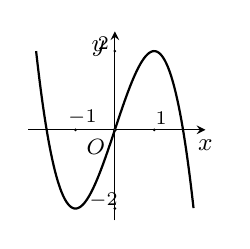
\begin{tikzpicture}[scale=.5]
\draw[-stealth] (-2.2,0) -- (2.3,0) node[below]{\small $x$};
\draw[-stealth] (0,-2.3) -- (0,2.5) node[below left]{\small $y$};
\draw[thick,smooth,samples=100] plot[domain=-2:2](\x,{-(\x)^3+3*(\x)});
\draw [fill=white,draw=black] (0,0) circle (1pt)node[below left]{\footnotesize $O$};
\foreach \x in{-1,1}\draw(\x,0) circle (.5pt) node[shift={(60:5pt)}]{\scriptsize $\x$};
\foreach \y in{-2,2}\draw(0,\y) circle (.5pt) node[shift={(145:5pt)}]{\scriptsize $\y$};
\end{tikzpicture}}
\end{ex} 
 
\begin{ex} 
 Trên đoạn $[1 ; 6]$, hàm số $y=x+\frac{9}{x+1}$ đạt giá trị nhỏ nhất tại điểm
\choice 
 { $x=1$} 
 { $x=8$} 
 { $x=2$} 
 { $x=6$}
\end{ex} 
 
\begin{ex} 
 Hàm số nào dưới đây đồng biến trên $(-\infty ;+\infty)$ ? 
 \choice 
{ $y=x^{3}+3 x-1$} 
 { $y=\frac{x}{x+2}$}
{ $y=x^{2}+1$} 
 { $y=x^{4}-2 x^{2}$}
\end{ex} 
 
\begin{ex} 
 Với mọi $a, b$ thỏa mãn $2 \log _{9} a-3 \log _{3} b=1$, mệnh đề nào dưới đây đúng?
\choice 
 { $a=\frac{3}{b^{3}}$} 
 { $2 a-3 b=1$} 
 { $a^{2}=3 b^{3}$} 
 { $a=3 b^{3}$}
\end{ex} 
 
\begin{ex} 
 Cho hình lập phương $A B C D \cdot A^{\prime} B^{\prime} C^{\prime} D^{\prime}$. Góc giữa hai đường thẳng $B A^{\prime}$ và $C C^{\prime}$ bằng
\choice 
 { $90^{0}$} 
 { $60^{0}$} 
 { $45^{0}$} 
 { $30^{0}$}
\end{ex} 
 
\begin{ex} 
 Nếu $\int_{2}^{4} f(x) d x=3$ thì $\int_{2}^{4}\left[f(x)-x^{3}\right] d x$ bằng
\choice 
 { $-57$} 
 { 63 } 
 { $-33$} 
 { $-237$}
\end{ex} 
 
\begin{ex} 
 Trong không gian $O x y z$, cho điểm $M(1 ;-2 ; 3)$ và mặt phẳng $(P): 2 x+y+z-1=0$. Đường thẳng đi qua điểm $M$ và vuông góc với mặt phẳng $(P)$ có phương trình là
 \choice
{ $\frac{x+2}{1}=\frac{y+1}{-2}=\frac{z+1}{3}$}
 { $\frac{x+1}{2}=\frac{y-2}{1}=\frac{z+3}{1}$} 
 { $\frac{x-1}{2}=\frac{y+2}{1}=\frac{z-3}{1}$} 
 { $\frac{x-2}{1}=\frac{y-1}{-2}=\frac{z-1}{3}$}
\end{ex} 
 
\begin{ex} 
 Cho số phức $z$ thỏa mãn $(1+i)(z-2)=4 i$. Phần ảo của số phức $\bar{z}$ bằng
\choice 
 { 4 } 
 { $-4$} 
 { 2 } 
 { $-2$}
\end{ex} 
 
 
\begin{ex} 
 Trong hộp có 30 tấm thẻ được đánh số thứ tự lần lượt từ số 1 đến số 30 . Người ta lấy ngẫu nhiên cùng một lúc từ hộp ra hai tấm thẻ rồi nhân số thứ tự của hai thẻ lấy được với nhau. Tính xác suất để tích thu được là một số chẵn.
\choice 
 { $\frac{1}{2}$} 
 { $\frac{22}{29}$} 
 { $\frac{7}{29}$} 
 { $\frac{51}{58}$}
\end{ex} 
 
\begin{ex} 
 Trong không gian $O x y z$, cho tứ diện $A B C D$ với $A=(2 ; 1 ; 2), B=(3 ; 2 ; 0), C=(1 ; 1 ; 3)$, $D=(-2 ; 2 ; 4)$. Mặt phẳng đi qua $D$ và song song với mặt phẳng $(A B C)$ có phương trình là
\choice 
 { $3 x-y+z+4=0$} 
 { $3 x+y+z=0$} 
 { $x+y+z-4=0$} 
 { $x-y+z=0$}
\end{ex} 
 
 \begin{ex} 
 Cho hình lăng trụ tam giác đều $A B C \cdot A^{\prime} B^{\prime} C^{\prime}$ với $A B=2$ và
$A A^{\prime}=3$. Tính khoảng cách $d$ từ điểm $A$ đến mặt phẳng $\left(A^{\prime} B C\right)$.
\choice 
 { $d=\frac{3}{2}$} 
 { $d=\frac{2}{3}$} 
 { $d=\frac{3}{\sqrt{13}}$} 
 { $d=\frac{6}{\sqrt{13}}$}
\end{ex} 

\begin{ex} 
 Cho hàm số đa thức bậc ba $y=f(x)$ có bảng biến thiên như sau:
\\ \centerline{

\begin{tikzpicture}
\tkzTabInit[nocadre,lgt=1.2,espcl=2.2]
{$x$ /.6,$f'(x)$ /.6,$f(x)$ /1.5}
{$-\infty$,$-1$,$2$,$+\infty$}
\tkzTabLine{,+,$0$,-,$0$,+,}
\tkzTabVar{-/ $-\infty$ ,+/$1$,-/$-5$,+/$+\infty$}
\end{tikzpicture}
}\\
Có bao nhiêu giá trị nguyên của tham số $m$ để phương trình $f^{\prime}(f(x)+m)=0$ có đúng bốn nghiệm thực phân biệt?
\choice
 { 4 } 
 { 5 } 
 { 0}
 { 6 }
\end{ex} 
 
\begin{ex} 
 Cho hàm số $y=f(x)$ có đạo hàm $f^{\prime}(x)$ thoả mãn $\left(1+x^{2}\right) f^{\prime}(x)-1=3 x^{4}+4 x^{2}, \forall x \in \mathbb{R}$ và $f(1)=0$. Biết $F(x)$ là một nguyên hàm của hàm số $21 . f\left(x^{2}\right)$ và $F(0)=10$, hãy tính $F(2)$
\choice
 { $F(2)=\frac{566}{21}$}
 { $F(2)=566$} 
 { $F(2)=366$} 
 { $F(2)=52$}
\end{ex} 
 
\begin{ex} 
 Cho khối chóp $S . A B C D$ có $S A \perp(A B C D)$. Đáy $A B C D$ là hình chữ nhật với $A B=a \sqrt{3}, A D=a$. Biết góc giữa hai mặt phẳng $(S A B)$ và $(S B D)$ bằng $45^{\circ}$, hãy tính theo $a$ thể tích $V$ của khối chóp $S . A B C D$ 
 \choice 
{ $V=\frac{\sqrt{2}}{2} a^{3}$} 
 { $V=\frac{\sqrt{2}}{6} a^{3}$}
{ $V=\frac{\sqrt{6}}{6} a^{3}$} 
 { $V=3 \sqrt{2} a^{3}$}
\end{ex} 
 
\begin{ex} 
 Trên tập hợp số phức, xét phương trình $z^{2}-2 z+m-3=0$ (với $m$ là tham số thực). Gọi hai điểm $A$ và $B$ là hai điểm biểu diễn hai nghiệm của phương trình đã cho. Biết rằng ba điểm $O, A, B$ là ba đỉnh của một tam giác vuông (với $O$ là gốc tọa độ), khẳng định nào dưới đây đúng?
\choice 
 { $m \in[3 ; 8)$} 
 { $m \in(-2 ; 3)$} 
 { $m \in[8 ; 10]$} 
 { $m \in(-6 ;-2]$}
\end{ex} 
 
\begin{ex} 
 Xét hai số phức $z_{1}, z_{2}$ thoả mãn $\left|z_{1}-3-5 i\right|=2$ và $\left|z_{2}+3+3 i\right|=3$. Gọi $M, m$ lần lượt là giá trị lớn nhất và giá trị nhỏ nhất của $\left|z_{1}-z_{2}\right|$, khi đó $M+m$ bằng
\choice 
 { 25 } 
 { 15 } 
 { 10 } 
 { 20 }
\end{ex} 
 
\begin{ex} 
 Cho khối nón đỉnh $S$ có đáy là hình tròn tâm $O$. Gọi $A$ và $B$ là hai điểm thuộc đường tròn đáy sao cho tam giác $S A B$ vuông và có diện tích bằng 16 . Góc tạo bởi giữa trục $S O$ và mặt phẳng $(S A B)$ bằng $30^{\circ}$. Thể tích của khối nón đã cho bằng
 \choice
{ $\frac{40 \sqrt{2}}{3} \pi$} 
 { $\frac{10 \sqrt{6}}{3} \pi$} 
 { $\frac{20 \sqrt{3}}{3} \pi$}
 { $\frac{40 \sqrt{3}}{3} \pi$}
\end{ex} 
 
\Closesolutionfile{ans}